\prob
{\label{t2:p7}
    Let $T_8$ and $R_8$ be the vector matroids of the following matrices over $GF(3)$:\pn
            \begin{center}
                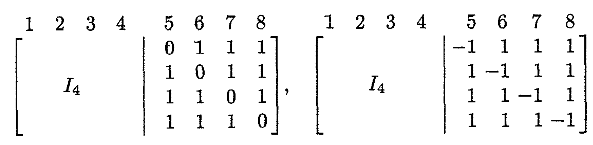
\includegraphics[width=12cm]{Test2/Problem7/FirstMatrices.png}
            \end{center}\pn
    
    \begin{enumerate}[label=(\roman*)]
        \item Show that $T_8$ and $R_8$ ar both self-dual.
        
        \item Show that $R_8$ is identically self-dual but $T_8$ is not.
        
        \item Give geometric representation for $T_8$ and $R_8$.
        
        \item Show that if $M \in \{T_8, R_8\}$ and $X = E(M) \setminus \{8\}$, then
                $(M|X)^* \cong F_7^-$.
                
        \item Consider the following matrices over $GF(3)$:
            \begin{center}
                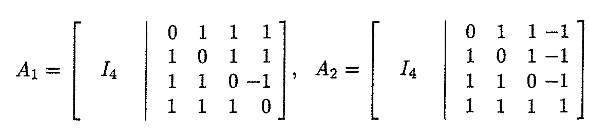
\includegraphics[width=12cm]{Test2/Problem7/SecondMatrices.png}
            \end{center}\pn
            Show, by applying a sequence of the row and clolumn opeartions to $A_1$ and $A_2$
            that $M[A_1] \cong T_8$ and $M[A_2] \cong R_8$.
            
        \item Show that $R_8$ can be obtained from $AG(3, 2)$ by relaxing two disjoint 
            circuit-hyperplanes.
    \end{enumerate}
}
\begin{proof}$\,$\pn
    \begin{enumerate}[label=(\roman*)]
        \item 
        
            Theorem 2.2.8 from~\cite{Oxley} sates that if a linear matroid is expresed as $[I_n | D]$,
            then its dual matroid can be represented with the matrix $[-D^T | I_r]$.\pn
            
            As multiplying columns by $-1$ doesn't change dependency/independency conditions. The dual matroid can be represented
            as $[D^T | I_r]$.\pn
            
            For both, $T_8$ and $R_8$, we have that $n = 4$, $r = 4$, and $D = D^T$. Then, in both cases, 
            $[D^T | I_4] = [D^T | I_4] = [D | I_4]$. And with this representation is clear how we would build an
            isomorphism from $T_8$ to $T_8^*$ and from $R_8$ to $R_8^*$.
            
        \item
            Lets write $T_8 = [I_4 | D_1]$, it is easy to prove that $T_8$ is not identically self-dual by
            simply pointing out a cobasis that is not a basis.\pn
            
            All the columns of $I_4$ form a basis. Then all the columns of $D$ form a cobasis, but such cobasis is
            dependent, if you sum up all of their columns you will get the zero vector.\pn
            
            Now lets show that $R_8$ is identically self-dual by showing that every cobasis is a basis. 
            For this, lets clasify the subsets of columns with cardinality 4 by how they intersect $I_4$.\pn
            
            There are three main types that intersect the columns in $I_4$
                \begin{enumerate}
                    \item \textbf{four columns from $I_4$.}
                        There is only one of these, and its complement (the columns from $D$) is also independent, its determinant
                        is $-16$ and $-16 \equiv 2 \mod 3$.
                        
                        So, in this case, every cobasis is basis.
                    \item \textbf{trhee columns from $I_4$ and one from $D$.}
                        Without loss of generality, lets say that the 3 columns from $I_4$ are the first three. If it is not the
                        case we can always exchange rows to make them look like the first three. Here are two subcases. The column
                        from $D$ is $8$ or it is $5$. If it is among $5, 6, 7$ we can always exchange rows to make them look
                        as if the column chosen from $D$ is 5.\pn
                        
                        If the column from $D$ is 8, the determinant of the columns $\{1, 2, 3, 8\}$ is -1, and the determinant of the complement
                        $\{4, 5, 6, 7\}$ is -4 and $-4 \equiv -1 \mod 3$.\pn
                        
                        If the column from $D$ is 5, the determinant of the columns $\{1, 2, 3, 5\}$ is 1, and the determinant of the complement
                        $\{4, 6, 7, 8\}$ is -4 and $-4 \equiv -1 \mod 3$.\pn
                        
                        Then, in this case, every cobasis is basis.\pn
                    \item \textbf{two columns from $I_4$ and two from $D$.}
                        Here are essentialy 3 subcases. And those are $\{1, 2, 5, 6\}$, $\{1, 2, 6, 7\}$ and $\{1, 2, 7, 8\}$. Any other can be
                        reduced to one of those by exchanging rows.\pn
                        
                        In the subcase $\{1, 2, 5, 6\}$ the determinant is 0. And the determinant of the complement $\{3, 4, 7, 8\}$ is 0 also.\pn
                        
                        In the subcase $\{1, 2, 6, 7\}$ the determinant is 2 which is $-1 \mod 3$. 
                        And the determinant of the complement $\{3, 4, 5, 8\}$ is -2, which is $1 \mod 3$.
                        
                        In the subcase $\{1, 2, 7, 8\}$ the determinant is 0. And the determinant of the complmement $\{3, 4, 5, 6\}$ is 0 also.\pn
                        
                        Then, in this case also, every cobasis is basis.\pn
                \end{enumerate}
                    
                The case \textbf{one colum from $I_4$ and three from $D$} is alredy covered in the complements of the case \textbf{trhee columns from $I_4$ and one from $D$.},
                Similarly, the case \textbf{four columns from $D$} is covered in the complement of the case \textbf{four columns from $I_4$}.
                
                Then, in any case, every cobasis is basis and then $R_8$ is identically self-dual.
        \item $\,$\pn
            \begin{figure}[H]
                \begin{center}
                    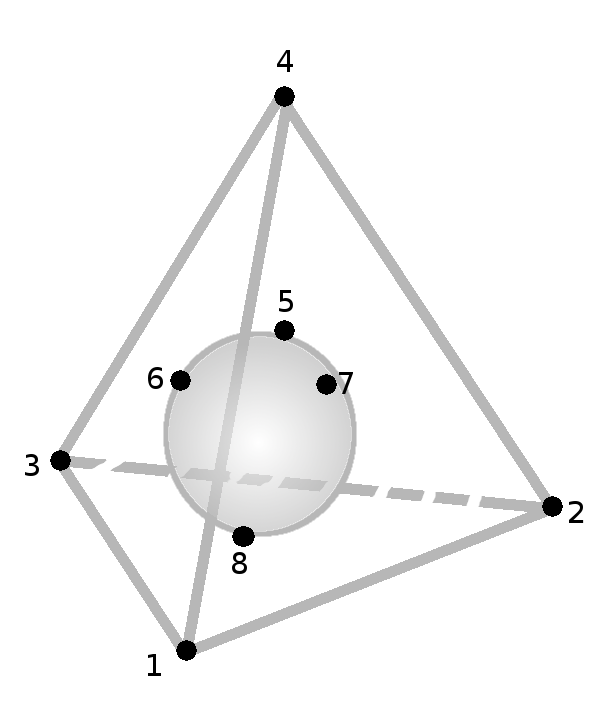
\includegraphics[width=8cm]{Test2/Problem7/T8GraphicRepresentation.png}
                \end{center}                            
                \caption{Geometric representation of T8}
                \label{t2:p7_T8GraphicRepresentation.png}                        
            \end{figure}\pn 
            
            In this representation, there are points in the center of each face of the thetrahedron and the sphere that is inside 
            the thetrahedron tangent to all the faces, is a plane that contains all the centers of the faces 
            (just as in Fano's plane the circle inside the triangle is a line).\pn
            
            Assuming that the thetrahedron is regular, all the other planes that have 4 vertices and that are not suggested in the
            figure are those that can be found in the euclidean space. For example $\{1, 2, 5, 6\}$.\pn
            
            \begin{figure}[H]
                \begin{center}
                    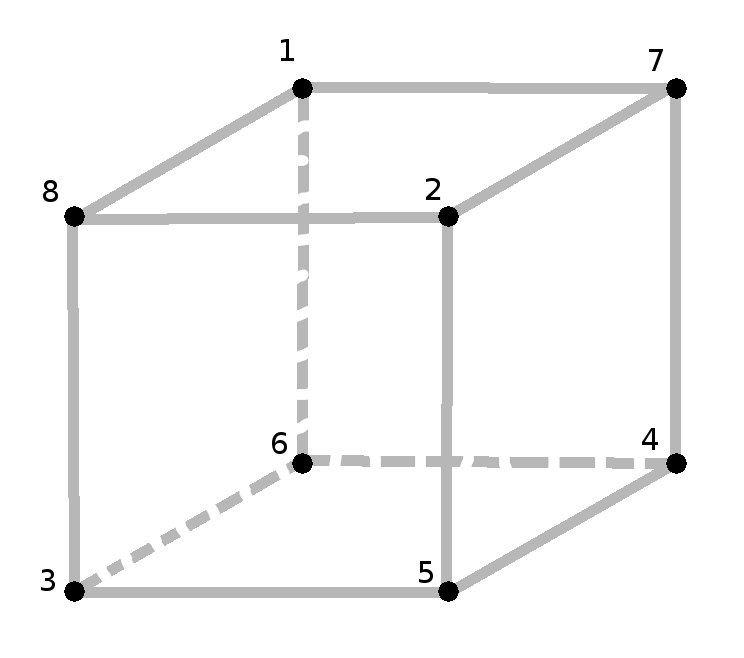
\includegraphics[width=8cm]{Test2/Problem7/R8GraphicRepresentation.png}
                \end{center}                            
                \caption{Geometric representation of $R_8$}
                \label{t2:p7_R8GraphicRepresentation.png}                        
            \end{figure}\pn 
            
            This representation is simply a cube. All the other planes that contain 4 vertices and that are not suggested in the figure 
            are those that can be found in the euclidean space. For Example $\{7, 8, 3, 4\}$.
        
        \item
            Given the first parenthesis of this excercise, we know that an isomorphism from $T_8$ to $T_8^*$ is given by simply
            sending 1 to 5, 5 to 1, 2 to 6, 6 to 2, 3 to 7, 7 to 3, 4 to 8, 8 to 4. Then we can relabel our geometric representation of
            $T_8$ and obtain one of $T_8^*$.
            
            \begin{figure}[H]
                \begin{center}
                    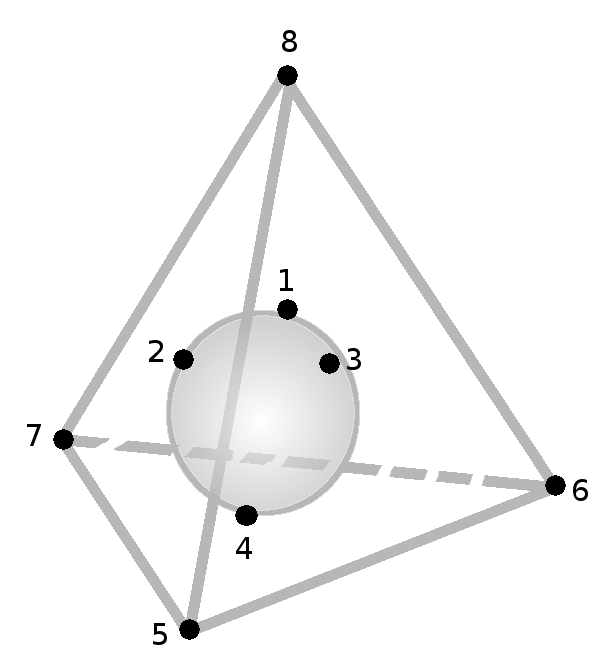
\includegraphics[width=8cm]{Test2/Problem7/T8DualGraphicRepresentation.png}
                \end{center}                            
                \caption{Geometric representation of $T_8^*$}
                \label{t2:p7_T8DualGraphicRepresentation.png}                        
            \end{figure}\pn 
                       
            We are being asked to contract $\{8\}$ in this representation. To contract is simply to create new circuits from those who
            contained the contracted elements, the new circuits will be those subsets that when we join $\{8\}$ to them, what we obtain
            is one of the old circuits.\pn
            
            In a geometric representation this is equivalent to ``getting rid of one dimension'', or projecting.\pn
            
            What we obtain from projecting with respect to 8, is the following representation.\pn
            
            \begin{figure}[H]
                \begin{center}
                    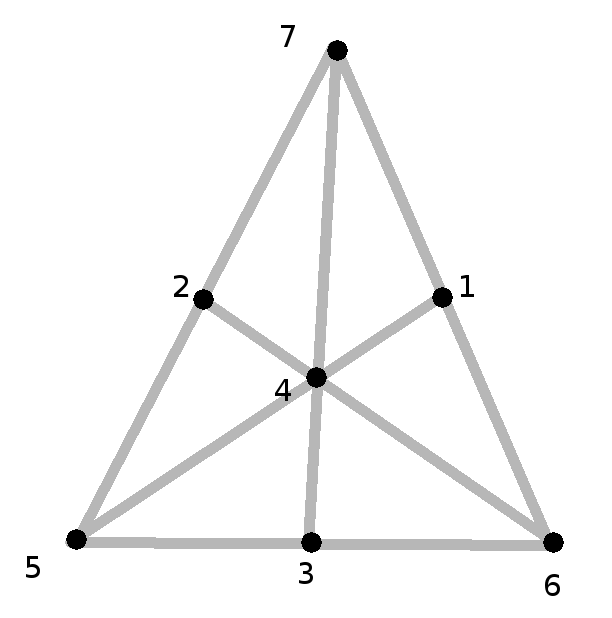
\includegraphics[width=6cm]{Test2/Problem7/T8DualMinorGraphicRepresentation.png}
                \end{center}                            
                \caption{Geometric representation of $T_8^* / \{8\}$}
                \label{t2:p7_T8DualMinorGraphicRepresentation.png}                        
            \end{figure}\pn 
            
            This is exactly the geometric representation of $F_7^-$.
            
            As $R_8$ is identically self-dual, the same representation from \ref{t2:p7_R8GraphicRepresentation.png} will work.\pn
            
            Then we must project from $8$ and se what is the result.
             \begin{figure}[H]
                \begin{center}
                    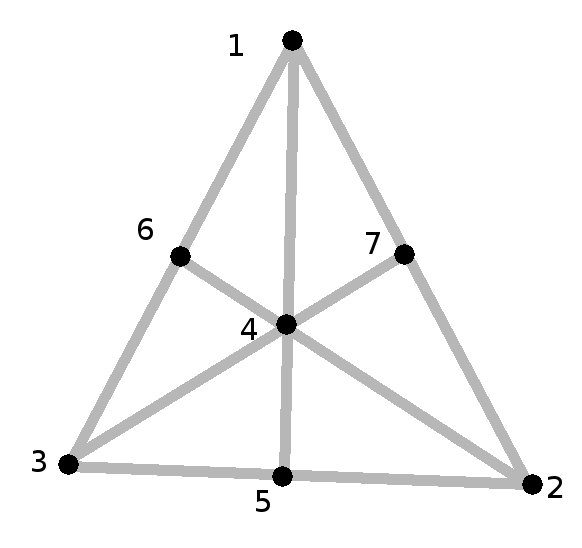
\includegraphics[width=6cm]{Test2/Problem7/R8DualMinorGraphicRepresentation.png}
                \end{center}                            
                \caption{Geometric representation of $R_8^* / \{8\}$}
                \label{t2:p7_R8DualMinorGraphicRepresentation.png}                        
            \end{figure}\pn 
            
            Which is againg the geometric representation of $F_7^-$.
            
        \item
            I have constructed a set of software tools to solve this parenthesis by brute force.\pn
        
            From the first parenthesis we know that all the basis and all the circuits in $T_8$ and $R_8$ have all
            exactly 4 elements.\pn
            
            I constructed a tool that looks in every of the 70 subsets of 4 columns in a $4 \times 8$ matrix and
            determines if it is a basis and another to determine if it is a circuit, both by taking the determinant modulo 3.\pn
            
            Then, to find an equivalence between $A_1$ and $T_8$, I made a another tool that will crawl among all
            the column permutations of $A_1$ and for each one determine the set of labels that are basis (or those that are circuits).\pn
            If such sets of labels are the same than in $T_8$, then we have an equivalency.\pn
            
            After such analysis, I found 24 permutations of the columns of $A_1$ that determines exactly the same matroid as $T_8$.\pn
            
            Exactly the same procedure will work for $A_2$ and $R_8$ and in that case, I found 96 permutations of the columns of $A_2$ that 
            give a matroid that is equivalent to $R_8$.\pn
            
            My first approach was to demonstrate that $A_1$ and $T_8$ where equivalent matrices and the same for $A_2$ and $R_8$.\pn
            
            In both cases, making use of gaussian-jordan elimination, I couldn't get the original matrices of $T_8$ and $R_8$. It
            would be not an elegant method, but I could determine that $A_1$ and $T_8$ are not equivalent and the same for
            $R_8$ and $A_2$ and it would take me a very long time to find any permutation that would work.\pn
            
            I will include my code here:
            
            This is the code that gives all the combinations of $m$ elements in a set of $n$ elements
            \small
                \lstinputlisting{Test2/Problem7/combinations.m}
            \normalsize
            
            This is the code that determines which are all the basis of the matroid, it works only
            if you give it the rank of the matroid, but it could be changed to determine it by itself.
            \small
                \lstinputlisting{Test2/Problem7/column_basis.m}
            \normalsize
            
            This is the code that determines which are all the circuits of the matroid, it works only if all
            the circuits have the same size (as in this case) and you give such size to the algorithm.
            \small
                \lstinputlisting{Test2/Problem7/column_circuits.m}
            \normalsize
            
            This is the code that crawls among all the permutations of one of the matrices and compares the set
            of basis with the set of basis of the other matrix.
            \small
                \lstinputlisting{Test2/Problem7/look_for_common_basis.m}
            \normalsize
       
            This is the code that crawls among all the permutations of one of the matrices and compares the set
            of circuits with the set of circuits of the other matrix.
            \small
                \lstinputlisting{Test2/Problem7/look_for_common_circuits.m}
            \normalsize
            
            This last two algoritmhs are redundant, but I made both just to double-check the results from
            any of them. With both, I obtained exactly the same set of permutations for both $A_1$ and $A_2$.\pn
            
            The result thrown by these algorithms is too long to be displayed here. But I'll include one case of
            each one.\pn
            
            $T_8$ is isomorphic to the matroid determined by:
            
            \[ \left( 
                \begin{array}{cccccccc}
                   0  & 0 &  1 &  1 &  0 &  0 &  1 &  1 \\
                   0  & 1 &  0 &  1 &  0 &  1 &  0 &  1 \\
                   1  & 0 &  0 &  0 &  0 &  1 &  1 & -1 \\
                   0  & 0 &  0 &  1 &  1 &  1 &  1 &  0
                \end{array} 
            \right)\] 
            
            Which is obtained from $A_1$ by permuting its columns.\pn
            
            $R_8$ is isomorphic to the matroid determined by:
            
            \[ \left( 
                \begin{array}{cccccccc}
                   0  & 0  & 1  &-1  & 0 &  0 &  1  & 1 \\
                   0  & 1  & 0  &-1  & 0 &  1 &  0  & 1 \\
                   1  & 0  & 0  &-1  & 0 &  1 &  1  & 0 \\
                   0  & 0  & 0  & 1  & 1 &  1 &  1  & 1
                \end{array} 
            \right)\] 
            
            Which is obtained from $A_2$ by permuting its columns.\pn
            
            
        \item
            $AG(3, 2)$ accepts the following representation, where every point
            is a vector in $\Z_2^3$
            
            \begin{figure}[H]
                \begin{center}
                    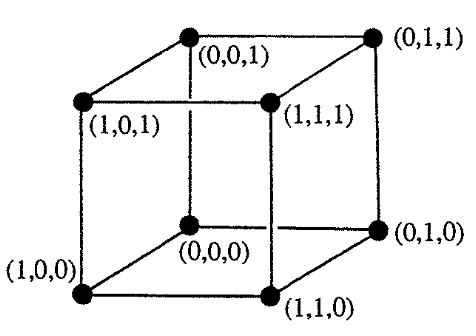
\includegraphics[width=6cm]{Test2/Problem7/AG_3_2.png}
                \end{center}                            
                \caption{Representation of $AG(3, 2)$}
                \label{t2:p7_AG_3_2.png}                        
            \end{figure}\pn 
            
            In this representation, every $4$ vertices that lay on the same plane are
            dependient. Any set of 3 vertices is independent. This can be seen by simply
            affinity in $\Z_2^3$.\pn
            
            There are also a pair of circuits that are not laying in a plane. And those are the
            two thetahedrons obtained by taking any vertex and all the neighbors of its antipode.
            
            By example let $T_1 = \{(0, 0, 0), (1, 1, 0), (1, 0, 1), (1, 1, 0)\}$.\pn
            
            It is complement is the other thetahedron. Both are circuits (If you sum them up, you will obtain
            the zero vector). Now, if you add the vector $(0, 0, 1)$ to $T_1$, you can generate $(1, 0, 0) = (1, 0, 1) + (0, 0 1)$,
            and you can generate $(0, 1, 0) = (1, 1, 0) + (1, 0, 0)$, and $(1, 0, 0) = (1, 1, 0) + (0, 1, 0)$, and
            $(1, 1, 1) = (1, 0, 0) + (0, 1, 0) + (0, 0, 1)$. Then $T_1$ is an hyperplane. It doesn't matter what you
            add to it, you are able to generate any other vector in $\Z_2^3$. The same will occur the other thetahedron.\pn
            
            Then, you can relax these two circuit-hyperplanes, and you will get exactly the representation of $R_8$ given in
            [\ref{t2:p7_R8GraphicRepresentation.png}].
    \end{enumerate}
\end{proof}